\section{L'équation de KdV}
\label{sec:KdV}
%%% Corrigé mais à revoir analyse d'echelle

\subsection{Le modèle}

\indent Le premier modèle de propagation d'ondes étudié et implémenté dans ce projet est l'équation de Korteweg-de Bries (KdV) , qui prend en compte les effets non linéaires et dispersives et qui est une bonne approximation pour des ondes de petite amplitude et grande longueur. \cite{BBM1971}

 \indent Plusieurs formes de cette équation peuvent être trouvées dans la littérature, variant notamment dans les coefficients d'échelle pour chacun des processus physiques présents dans l'équation (non linéarité et dispersion). On considère la formulation présentée par \cite{BBM1971}, écrite en termes de variables sans dimensions mais non échallonées : 

\begin{equation*}
    u_t + u_x + (u^2)_x + u_{xxx} = 0
\end{equation*}

\subsection{Discrétisation}

\indent Le problème qu'on veut résoudre, avec une condition initiale $\Phi$ et des conditions aux bords appropriées, est

\begin{equation*}
\begin{cases}
    u_t + u_x + (u^2)_x + u_{xxx} = 0 \ , \ \ x \in [x_{min},x_{max}], \ \ t \in [0, t_{max}] \\
    u(x,0) = \Phi(x) \\
    \text{+ boundary conditions}
\end{cases}
\end{equation*}

\indent Dans un premier moment, pour valider l'implémentation du modèle, sans influence des bords, on considère des conditions aux bords périodiques, ou des conditions de Dirichlet et/ou de Neumann homogènes mais suffisamment éloignées de l'onde (c'est-à-dire, du support de la solution).

\indent La résolution numérique du problème est faite avec un schéma de \emph{splitting}, en séparant les termes d'advection et de dispersion. Alors, en définissant les opérateurs

\begin{equation*}
	T_a(u) = u_t + u_x + (u^2)_x, \qquad
	T_d(u) = u_t + u_{xxx}
\end{equation*}

 \noindent on résout, dans chaque pas de temps $[t_n,t_{n+1}]$ :
 
\begin{equation*}
\begin{cases}
   T_a(v) = 0 \ \ ,\ t \in [t_n,t_{n+1}], \  v^n = u^n \\
   T_d(w) = 0 \ \ , \ t \in [t_n,t_{n+1}], \  w^n = v^{n+1} \\
    u^{n+1} = w^{n+1}
\end{cases}
\end{equation*}

\indent Les schémas numériques utilisés dans chacun de ces pas son décrites ci-dessous :

\subsubsection{Premier pas du \emph{splitting} - advection}
\label{sec:KdVSplitted1}

\indent Le premier pas du schéma de splitting pur l'équation de KdV est une loi de conservation hyperbolique, qui peut être écrite en termes d'une fonction de flot $f$ :

\begin{equation}
  \label{eq:conservationLaw}
	v_t + f(v)_x = 0,  \qquad f(v) = v + v^2
\end{equation}

\indent Cette équation est résolue avec une méthode de volumes finis, où les cellules $[x_{i-1/2}, x_{i+1/2}]$ sont centrées dans les points discrets $x_i$ et avec des valeurs moyens de $u$ égales à la solution dans ces points. La dérivée spatiale dans \eqref{eq:conservationLaw} est discretisée avec une méthode de Runge-Kutta d'ordre 4 :

\begin{equation*}
\begin{gathered}
k_1 = - f(v_i^n)_x, \qquad
k_2 = - f\left(v_i^n + k_1\frac{\Delta t }{2}\right)_x \\
k_3 = - f\left(v_i^n + k_2\frac{\Delta t }{2}\right)_x, \qquad
k_4 = - f(v_i^n + k_3 \Delta t)_x \\
v_i^{n+1} = v_i^n + \frac{\Delta t}{6}(k_1 + 2k_2 + 2k_3 + k_4)
\end{gathered}
\end{equation*}

\noindent et la dérivée spatiale est approximée en termes du flot dans les interfaces de las cellules :

\begin{equation*}
f(v_i^n)_x = \frac{f\left(v_{i+1/2}^n\right) - f\left(v_{i-1/2}^n\right)}{\Delta x}
\end{equation*}

\indent Alors, il faut calculer las valeurs de $u$ dans chaque interface. Cela sera fait en résolvant le problème de Riemann suivant :

\begin{equation*}
\begin{cases}
v_t + f(v)_x = 0 \\
v(x,0) = v^- \ , \ x < 0 \\
v(x,0) = v^+ \ , \ x > 0
\end{cases}
\end{equation*}

\noindent où l'interface se trouve dans $x=0$ et $v^-$ et $v^+$ sont les solutions dans les cellules voisines.

\indent La fonction de flot $f$ es uniformément convexe; alors le problème de Riemann a une unique solution faible admissible  \cite{conservationLaws2002} :

\begin{itemize}
\item  If $v^- > v^+$  (choc) : 
\begin{equation*}
v(x,t) = 
\begin{cases}
v^- \ ,\ \   f(v^-) > f(v^+) \\
v^+ \ ,\ \ f(v^-) < f(v^+)
\end{cases}
\end{equation*}

\item If $v^+ > v^-$  (onde de raréfaction) :
\begin{equation*}
v(x,t) = 
\begin{cases}
v^- \ ,\ \ f'(v^-) > 0 \\
\left(f'\right)^{-1}(v) \ ,\ \ f'(v^-) < 0 < f'(v^+) \\
v^+ \ ,\ \ f'(v^+) < 0 
\end{cases}
\end{equation*}
\end{itemize}


\subsubsection{Deuxième pas du \emph{splitting} - dispersion}

\indent Deux schémas sont proposés pour la résolution du deuxième pas de l'équation de KdV :

\begin{equation}
	\label{eq:dispersion}
	w_t + w_{xxx} = 0
\end{equation}

\noindent en dépendant des conditions aux bords (périodiques ou pas).

\paragraph{Le cas périodique}

\indent Les dérivées spatiales et la linéarité de l'équation \eqref{eq:dispersion} nous motivent à mettre en ouvre une méthode spectrale de Fourier, ce qui est possible avec des conditions aux bords périodiques. En fait, la méthode est assez simple :

\indent Soit $\hat{w}(k,t_n)$  les coefficients de Fourier de $w(x,t_n)$. La transformée de Fourier de l'équation \eqref{eq:dispersion} fournit

\begin{equation*}
	\hat{w}_t(k,t) - ik^3\hat{w}(k,t) = 0
\end{equation*}

\indent C'est une EDO dans $t$, dont la solution est

\begin{equation*}
\hat{w}(k,t) = e^{ik^3(t-t_n)}\hat{w}(k,t_n)
\end{equation*}

\indent Finalement, la transformée inverse de Fourier utilisant les coefficients $\hat{w}(k,t_{n+1})$ donne $w(x,t_{n+1})$.

\paragraph{Le cas non périodique}

\indent Dans ce cas, on discrétise l'équation \eqref{eq:dispersion} avec un schéma de différences finies implicite de quatrième ordre pour la troisième dérivée spatiale, sauf dans les points les plus proches des bords, pour lesquels un schéma décentré  d'ordre 1 est utilisé :

\begin{equation*}
\begin{gathered}
	\frac{u_i^{n+1} - u_i^n}{\Delta t} + \frac{\frac{1}{8}u_{i-3}^{n+1} - u_{i-2}^{n+1}  + \frac{13}{8}u_{i-1}^{n+1} - \frac{13}{8}u_{i+1}^{n+1} + u_{i+2}^{n+1} - \frac{1}{8}u_{i+3}^{n+1}}{\Delta x^3} = 0, \ \ i = 3,...,N-3 \\
	\frac{u_i^{n+1} - u_i^n}{\Delta t}  + \frac{-u_{i}^{n+1} + 3u_{i+1}^{n+1}  -3 u_{i+2}^{n+1} + u_{i+3}^{n+1} }{\Delta x^3} = 0, \ \ i = 0,1,2 \\
	\frac{u_i^{n+1} - u_i^n}{\Delta t}  + \frac{u_{i}^{n+1} - 3u_{i-1}^{n+1}  + 3 u_{i-2}^{n+1} - u_{i-3}^{n+1} }{\Delta x^3} = 0, \ \ i = N-2,N-1,N 
\end{gathered} 
\end{equation*}

\indent Cette discrétisation ramène à la résolution d'un système linéaire, pour lequel on fait les modifications appropriées pour prendre en compte les conditions aux bords.

\subsubsection{Choix de la taille de maille}

\indent On a implémenté les méthodes décrites ci-dessus avec un pas de temps variable, choisi en se basant sur le premier pas du schéma de \emph{splitting}. Dans la forme non conservative, l'équation \eqref{eq:conservationLaw} peut être écrite comme

\begin{equation*}
v_t +  (1+2v)v_x = 0
\end{equation*}

\noindent ce qui s'agit d'un problème d'advection avec une vitesse $1+2v$.

\indent Les pas spatial et temporal doivent vérifier la condition CFL :

\begin{equation*}
(1+2v)\frac{\Delta t}{\Delta x} \leq 1
\end{equation*}

\noindent pour éviter des comportements non physiques (e.g. création de masse). Alors, dans chaque pas de temps, on choisit, pour un $\epsilon$ petit :

\begin{equation*}
\Delta t = \frac{\Delta x}{1+2\max\limits_{x}|v|} - \epsilon
\end{equation*}

\subsection{Analyse d'échelle}

\indent En envisageant la correcte simulation des phénomènes physiques qui jouent un rôle dans l'équation de KdV, la solution initiale doit satisfaire les hypothèses faites lors de la dérivation du modèle. Ayant cet objectif en tête, on fait dans les paragraphes suivants une analyse d'échelle en suivant les arguments présentés par \cite{BBM1971}. Cette analyse nous permettra d'étudier la validité physique du modèle et de dériver un critère pour sélectionner les conditions initiales pour quelques exemples de simulations numériques.

\indent On veut écrire l'équation de KdV dans la forme suivante (sans dimension et échallonée), selon la description de \cite{BBM1971} :

\begin{equation}
\label{eq:scaledKdV}
U_T + U_X + \frac{\epsilon}{2} (U^2)_X + \epsilon\alpha^2U_{XXX} = 0
\end{equation}

\noindent et la lier aux paramètres du modèle d'ondes de surface dans forme dimensionnelle \cite{Khorsand2014}

\begin{equation}
\label{eq:physiqueKdV}
    u^*_{t^*} + c_0u^*_{x^*} + \frac{3}{4}\frac{c_0}{h_0}({u^*}^2)_{x^*} + \frac{1}{6}c_0h_0^2u^*_{x^*x^*x^*} = 0 
\end{equation}

\noindent où $\cdot^*$ indique les variables physiques, $h_0$ la profondeur de l'eau non perturbée pour un fond plat, et $c_0 = \sqrt{gh_0}$ la vitesse d'onde longue.

%\subsubsection{Caractérisation de la non linéarité}
%
%\indent D'après \cite{BBM1971}, la non linéarité est caractérisée par un paramètre $\epsilon$ tel que les caractéristiques sont écrites dans la forme
%
%$$ \frac{1}{c_0} \frac{dx^*}{dt^*} = 1+ bu^*$$
%
%\noindent alors on peut choisir un $\epsilon \ll 1$ tel que  $bu=\epsilon U$, avec $u$ d'ordre 1. Pour le cas particulier d'ondes d'eau, ceci peut être représenté par
%
%$$ \frac{1}{c_0} \frac{dx}{dt} = 1 + \frac{3}{2h_0}u$$
%
%\noindent alors 
%
%\begin{equation}
%\label{eq:analysisb}
%b = \frac{3}{2h_0}
%\end{equation} 
%
%\indent Ce paramètre sera utilisé dans les arguments suivants.
%
%\subsubsection{Caractérisation de la dispersion}


\indent D'après \cite{BBM1971}, la non linéarité est caractérisée par un paramètre $\epsilon \ll 1$ tel que les caractéristiques sont écrites dans la forme

$$ \frac{1}{c_0} \frac{dx^*}{dt^*} = 1+ bu^*$$

\noindent et $bu*=\epsilon U$, avec $u$ d'ordre 1. 


\indent La caractérisation de la dispersion, à son tour, vient de la dérivation de l'équation de KdV. D'après \cite{BBM1971}, si la propagation de l'onde suit une loi de la forme

$$ u^*_{t^*} + u^*u^*_{x^*}+(\mathcal{L} u^*)_{x^*} = 0$$

\noindent avec $\mathcal{L}$ tel que $$ \widehat{\mathcal{L}u^*} = \frac{c(k)}{c_0} \widehat{u^*}(k,t)$$ où $\hat \cdot$ dénote la transformée de Fourier et  $c(k)$ la célérité  de phase, alors, pour $\kappa$ suffisamment petit, la vitesse d'onde

\begin{equation}
\label{eq:expansionc}
c(\kappa) = c_0 + c_0 \sum_{n=1}^{\infty}A_n\epsilon^n\kappa^{2n}
\end{equation}

\noindent peut être approximée par  $c(\kappa) = c_0(1-\kappa^2)$, ce qui motive les remplacements $ X=\sqrt{\epsilon}x^*$, $T =c_0 \sqrt{\epsilon} t^*$, et $u^* = \frac{\epsilon}{ b} U$ pour obtenir l'équation équivalente   

%, ce qui est équivalent à

%$$ \mathcal{L} u = \mathcal{F}^{-1}\left(\frac{c(k)}{c_0}\right) * u$$ 

%\noindent où $\mathcal{F}^{-1}$ es l'opérateur de la transformée inverse de Fourier,


\begin{equation}
\label{eq:scaledEquation}
 U_T + \epsilon U U_x+(\mathcal{L}_{\epsilon} U)_{X} = 0
 \end{equation}

\noindent avec $\mathcal{L}_\epsilon$ tel que 

\begin{equation}
\label{eq:operatorL}
\widehat{\mathcal{L}_\epsilon U} = \frac{c(\epsilon^{1/2} K)}{c_0} \hat{U}(K,T)
\end{equation}

\noindent où $K=\sqrt{\epsilon} k$. Après le remplacement de l'expansion \eqref{eq:expansionc} dans \eqref{eq:operatorL}, on obtient

\begin{align}
  \label{eq:expansionLe}
    \mathcal{L}_\epsilon U &=U +\sum_{n=1}^\infty (-1)^n A_n \epsilon^n \partial_X^{2n} U    
\end{align}

\noindent et si les termes pour $n\geq2$ sont négligeables (ce qui est le cas pour $\epsilon \ll 1 $) et si on suppose que toutes les dérivées de $U$ sont de la même ordre de magnitude, alors on obtient

\begin{equation*}
    \mathcal{L}_\epsilon U = U + A_n \epsilon \frac{\partial^2 U}{\partial x^2} = U - \alpha^2 \epsilon \frac{\partial^2 U}{\partial x^2}
\end{equation*}

\noindent avec $\alpha^2 = - A_n$. En remplaçant dans l'équation échelonnée \eqref{eq:scaledEquation}, on obtient

$$U_T + U_X + \frac{\epsilon}{2} (U^2)_X + \epsilon\alpha^2U_{XXX} = 0$$

\indent L'application du même échelonnement $ X=\sqrt{\epsilon}x^*$, $T =c_0 \sqrt{\epsilon} t^*$, et $u^* = \frac{\epsilon}{ b} U$ à l'équation physique \eqref{eq:physiqueKdV} fournit $$U_T + U_X + \frac{3\epsilon}{4h_0b} (U^2)_X + \frac{h_0^2\epsilon}{6}U_{XXX} = 0$$ 

\noindent d'où, en comparant avec  \eqref{eq:scaledKdV}, on conclue que 

\begin{equation}
\label{eq:analysisb}
b = \frac{3}{2h_0}, \qquad \alpha^2 = \frac{h_0^2}{6}
\end{equation} 


\subsection{Le critère pour choisir une solution initiale appropriée}

\indent En se basant sur l'analyse d'échelle faite ci-dessus, on va proposer un critère pour choisir des conditions initiales (i.e., la longueur et l'amplitude de l'onde initiale) pour lesquelles l'équation de KdV est physiquement valide. 

\subsubsection{Choix de la longueur d'onde}

\indent Une condition suffisante pour que les termes d'ordre supérieur à 1 dans l'expansion en série de potences de $\mathcal{L}_\epsilon$  (équation \ref{eq:expansionLe}) soient négligeables es que ces termes soient aussi négligeables pour $c(k)$ (dans l'équation \ref{eq:expansionc}), étant donné que toutes les dérivées de $U$ aient ordre de magnitude 1 (une assomption faite par \cite{BBM1971}).

\indent  D'après \cite{BBM1971}, l'expression suivante est applicable à des ondes de surface :

$$c(\kappa) = c_0 \left(\frac{tanh(\kappa h_0)}{\kappa h_0}\right) = c_0 \left(1 - \frac{1}{6}(\kappa h_0)^2 + \frac{19}{360}(\kappa h_0)^2 + ... \right) $$

\noindent d'où on voit qu'il faut choisir $\kappa h_0 \ll 1$ pour que les dérivées d'ordre $n>1$ soient négligeables.

\indent En dénotant la longueur d'onde par $\lambda$, et en choisissant une constante $B$ telle que $\kappa h_0  =  B \ll 1$, on a que $$h_0 = \frac{B\lambda}{2\pi}$$ et, de la relation $\alpha^2 = \frac{h_0^2}{6}$, on obtient $\alpha^2 = \frac{B^2\lambda^2}{6(2\pi)^2}$.

\subsubsection{Choix de l'amplitude de l'onde}

\indent Du changement de variables $bu^* = \epsilon U$, avec $U$ d'ordre de magnitude 1, et en considérant $b = \frac{3}{2h_0}$ (expression \ref{eq:analysisb}), la variable physique est écrite comme $u^* = \frac{2}{3}h_0\epsilon U, \ (\epsilon > 0)$. Alors

\begin{equation*}
A = \frac{2}{3}\epsilon h_0
\end{equation*}

\noindent est l'amplitude de l'onde. La détermination de l'amplitude est faite en considérant $\epsilon \ll 1$. 

\subsubsection{Résumé}

\indent Alors, le critère proposé ici pour construire la condition initiale pour l'équation de KdV est 

\begin{enumerate}
\item Adopter une profondeur $h_0$ (e.g. à partir des données disponibles);
\item Choisir une amplitude d'onde $A = \frac{2}{3}h_0\epsilon$, alors la restriction $\epsilon \ll 1$ ramène à $\frac{A}{h_0} = \frac{2}{3}\epsilon \ll 1$.
\item Choisir une longueur d'onde $\lambda$ telle que $\kappa h_0 = \frac{2\pi}{\lambda}h_0 = B \ll 1$, ce qui ramène à $\frac{h_0}{\lambda} = \frac{B}{2\pi} \ll 1$
\item L'effet de dispersion sur la non linéarité peut être mesurée par le quotient des respectifs coefficients, $\frac{\epsilon \alpha^2}{\epsilon} = \alpha^2$.
\end{enumerate}

\indent D'un autre point de vue, on peut définir une onde d'amplitude  $A$ et longueur $\lambda$ et déterminer l'intervalle de profondeurs dans lequel cette condition initiale est valide, pour une précision $(\epsilon,B)$ donnée :

\begin{equation} 
\label{eq:hvalid}
h_0^{valid} = \left[ \frac{3A}{2\epsilon}, \frac{B\lambda}{2\pi}\right]
\end{equation}

\noindent ce qui est consistant avec le fait de que le modèle de KdV est valide pour des ondes de petite amplitude et grande longueur \cite{BBM1971}.

\subsection{Tests numériques}

\indent On présente ci-dessous deux examples pour tester la résolution numérique proposée pour l'équation de KdV. Ces exemples sont inspirés dans ceux présentés dans \cite{conservationLaws2002}: les solutions initiales sont des gaussiennes (la solution est non périodique, mais suffisamment lointaine des bords afin d'éviter son influence) avec des différentes amplitudes et longueurs (la longueur d'onde est adoptée comme étant l'écart standard). L'idée est de vèrifier l'influence de ces caractéristiques sur les effets non linéaires et dispersives, et aussi de vérifier le range de profondeur d'eau dans lequel la propagation de chaque solution peut être modelée par l'équation de KdV (selon l'expression \ref{eq:hvalid}). Les deux tests ont été faits en considérant $B = 0.1$ et $\epsilon = 0.001$.

\indent Les solutions initiales utilisées sont

\begin{enumerate}
	\item \textbf{Onde courte (figure \ref{fig:KdVcriteriaShort})} % Criteria 6
		\begin{itemize}
			\item $\lambda = 1$
			\item $ A = 10^{-5}$
			\item $ h_0^{valid} = [0.15, 0.16] $
		\end{itemize}
	\item \textbf{Onde longue (figure \ref{fig:KdVcriteriaLong})} % Criteria 5
		\begin{itemize}
			\item $\lambda = 250000$
			\item $ A = 0.1$
			\item $ h_0^{valid} = [150, 3979] $
		\end{itemize}
\end{enumerate}

\indent La figure \ref{fig:KdVcriteria} présente les solutions dans quelques instants de simulation :

\begingroup
\addtocounter{figure}{1}
\begin{minipage}[t]{\linewidth}
\begingroup
\begin{minipage}[t]{.45\linewidth}
		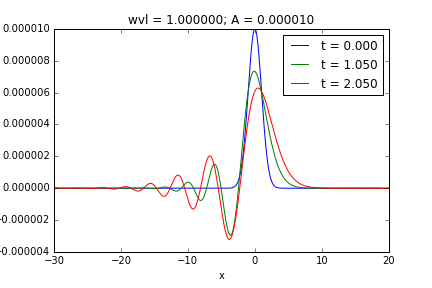
\includegraphics[scale=.45]{figures/criteria6.png}
		\captionof{subfigure}{Onde gaussienne courte \label{fig:KdVcriteriaShort}}
	\end{minipage}
\endgroup
	\hfill
\begingroup
	\begin{minipage}[t]{.5\linewidth}
		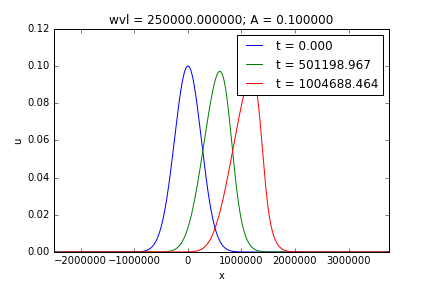
\includegraphics[scale=.45]{figures/criteria5.png}
		\captionof{subfigure}{Onde gaussienne longue		\label{fig:KdVcriteriaLong}}
	\end{minipage}
	\addtocounter{figure}{-1}
	\captionof{figure}{Simulations avec l'équation de KdV  	\label{fig:KdVcriteria}}
\endgroup
\end{minipage}
\endgroup

\paragraph{Conclusions partiales :}


\begin{itemize}
 \item Les resultats obtenus sont cohérents avec les observations et exemples faits par \cite{conservationLaws2002}, qui affirme que les effets dispersives sont plus fortes dans des ondes plus courtes; pour des ondes plus longues, les effts non linéaires sont plus évidents.
 \item Le range de validité de l'équation de KdV est très petit dans le cas de l'onde courte, et beaucoup plus grand dans le cas de l'onde large, ce qui est cohérent avec la validité du modèle de KdV pour les ondes de petite amplitude et grande longueur. Cela peut être observé dans la définition de $h_0^{valid}$ (équation \eqref{eq:hvalid}) : en réduisant $A$ et augmentant $\lambda$, la taille du range de validité augmente.
 \item Néanmoins, on n'a pas validé une des conclusions qu'on a faites lors de la dérivation du critère proposé. On a affirmé que l'importance relative des effets dispersives et non linéaires peut être mesurée par $\alpha^2 = \frac{h_0^2}{6}$ , mais, dans les exemples testés, si on adopte $h_0$ comme étant la médiane de $ h_0^{valid} $, l'onde courte (qui est très dispersive) a un $\alpha^2$ plus petite que l'onde large.
\end{itemize} 
